\begin{figure}[!ht]
    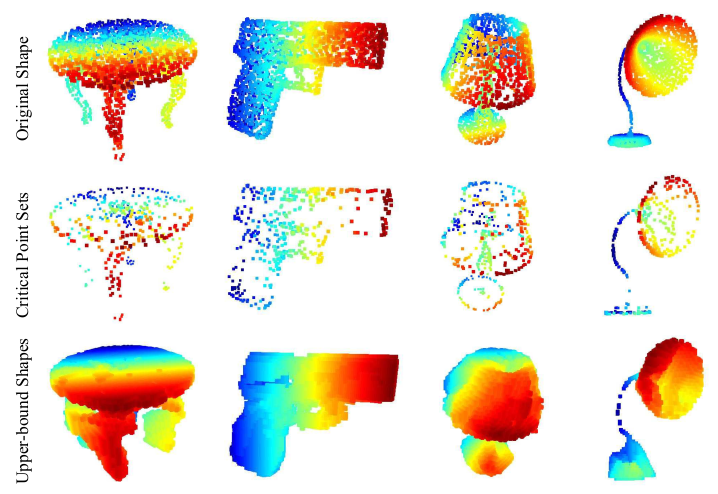
\includegraphics[width=0.5\textwidth]{critical_points}
    \caption{
        \textbf{Critical points and upper bound shape.} The critical point set
        together fully determines the global feature description for a given
        shape. Any point cloud between the critical point set and the upper
        bound shape gives exactly the same feature description. All figures are
        color-coded to provide depth information.
        Figure from \cite{qi2017pointnet}.
        % "\textbf{Critical points and upper bound shape.} While critical points
        % jointly determine the global shape feature for a given shape, any point
        % cloud that falls between the critical points set and the upper bound
        % shape gives exactly the same feature. We color-code all figures to show
        % the depth information." Figure and caption taken from \cite{qi2017pointnet}.  \todo{rewrite in own words}
    } \label{fig:critical_points}
\end{figure}


